\documentclass[11pt,a4paper]{article}

\usepackage{../../templates/style}

\begin{document}

\begin{problem}{Longest}{standard input}{standard output}{1 second}{64 megabytes}


แผ่นวงจรสี่เหลี่ยมขนาดกว้าง $M$ หน่วย ยาว $N$ หน่วย ถูกแบ่งเป็นช่องสี่เหลี่ยมจัตุรัส $M \times N$ ช่อง แต่ละช่องอาจเคลือบด้วยโลหะพิเศษ หรือเป็นช่องธรรมดา

เราต้องการวางลวดตัวนำยิ่งยวดลงบนแผ่นวงจรดังกล่าว โดยมีเงื่อนไขดังนี้
\begin{enumerate}

\item ลวดตัวนำจะต้องวางอยู่บนช่องที่เคลือบโลหะพิเศษเท่านั้น
\item ลวดตัวนำสามารถงอเป็นมุมฉากได้หนึ่งครั้ง
\item ถ้าลวดตัวนำวางลงบนแผ่นวงจรช่องใด ลวดจะต้องวางผ่านที่จุดกึ่งกลางของช่องนั้นเสมอ
\end{enumerate}

รูปด้านล่างแสดงตัวอย่างการวางลวดตัวนำบนแผ่นวงจรขนาด $4 \times 5$ (ช่องสีขาวแทนช่องที่มีโลหะพิเศษ ช่องดำคือช่องธรรมดา)

\begin{figure}[h!]
\centering
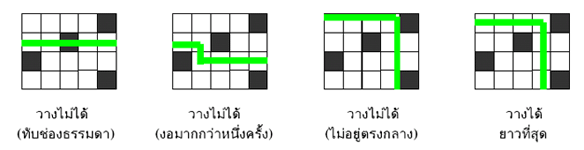
\includegraphics[width=1\textwidth]{../latex/img/1058/1058-1.png}
\end{figure}

เราต้องการทราบความยาวที่มากที่สุดของลวดตัวนำที่สามารถวางลงไปบนแผนวงจรได้


\bigskip
\underline{\textbf{โจทย์}}  ให้เขียนโปรแกรมรับจำานวนแผ่นวงจร จากนั้นสำหรับแต่ละแผ่นวงจร ให้เขียนโปรแกรมรับข้อมูลของการเคลือบแต่ละช่องของแผ่นวงจรนั้นแล้วคำนวณหาความยาวที่มากที่สุดของลวดตัวนำที่สามารถวางลงไปบนแผนวงจรได้

\InputFile

\textbf{บรรทัดแรก} ระบุจำนวนเต็ม $K$ แทนจำนวนแผ่นวงจรที่มี $(1\leq K\leq 5)$ จากนั้นข้อมูลนำเข้าจะประกอบด้วยข้อมูล $K$ ชุด แผ่นละหนึ่งชุด

\textbf{สำหรับแต่ละชุด}

\textbf{บรรทัดแรกของชุดนั้น} ระบุจำนวนเต็ม $M$ และ $N$ $(1 \leq M \leq 1\,000; 1 \leq N \leq 1\,000)$ 

\textbf{บรรทัดที่ $2$ ถึง $M+1$ ของชุดนั้น }จะระบุข้อมูลของแผ่นวงจร โดยในบรรทัดที่ $i+1$ สำหรับ $1 \leq i \leq M$ จะมีสตริง $A_i$ ความยาว $N$ ตัวอักษร ระบุข้อมูลของแผ่นวงจรในแถวที่ $i$ ตัวอักษรตัวที่ $j$ ใน $A_i$ จะมีค่าเป็น $1$ ถ้าช่องที่ $j$ เป็นช่องที่เคลือบโลหะพิเศษ และเป็น $0$ ถ้าช่องที่ $j$ เป็นช่องธรรมดา


\OutputFile

\textbf{มี $K$ บรรทัด} แต่ละบรรทัดระบุจำานวนเต็มแทนความยาวของลวดตัวนำที่มากที่สุด สำหรับข้อมูลของแผ่นวงจรแต่ละชุด

\Examples

\begin{example}
\exmp{2
4 5
11110
11011
01111
11110
2 5
01110
11000}{7
4}%
\end{example}

\Scoring

\textbf{ในข้อมูลชุดทดสอบที่มีคะแนนรวมไม่น้อยกว่า 70\%}:  $K \leq 2; N \leq 500; M \leq 500$


\Source

Young Thai Online Programming Competition 2008

\end{problem}

\end{document}